% Drawing 144/07-4 -- folder 144, batch 07, archive page 133 (PDF page 134).
% Transcription: un diagramme en perspective d'inclusions de sous-groupes, chaque flèche à crochet marquée de son indice : $\{1\}\overset{2}{\hookrightarrow}\mu$, $\{1\}$ et $\mu_{\tau'}$ reliés par un trait d'indice 2, $\mu_{\tau'}\overset{2}{\hookrightarrow}D_{\tau'}$, $\mu$ et $D_{\tau'}$ reliés par un trait d'indice 2 ; $D_{\tau'}\overset{2}{\hookrightarrow}D_\sigma$, $D_{\tau'}\hookrightarrow\Pi_{\tau'}$, $D_{\tau'}\overset{3}{\hookrightarrow}D_\rho$ ; $\mu\overset{2}{\hookrightarrow}L_\sigma$, $\mu\hookrightarrow\underline{\Pi}$, $\mu\overset{3}{\hookrightarrow}L_\rho$ ; $L_\sigma$ et $\Pi_{\tau'}$ reliés par un trait d'indice 2, $L_\sigma$ et $\underline\Pi$ de même, $L_\rho$ et $D_\rho$ (indice 2) ; $\Pi_{\tau'}\overset{6}{\hookrightarrow}\mathfrak{S}$, $D_\sigma\hookrightarrow\mathfrak{S}$, $D_\rho\hookrightarrow\mathfrak{S}$, $D_\rho\overset{6}{\hookrightarrow}\underline{\mathfrak{S}}^+$, $L_\rho\hookrightarrow\underline{\mathfrak{S}}^+$, $\mathfrak{S}$ et $\mathfrak{S}^+$ reliés par un trait d'indice 2. Des étiquettes au crayon, $SD_\sigma$ et $SZ_\sigma$, sont esquissées.
% Kind: perspective diagram of subgroup inclusions with indices (I). Method 2 (schematic redraw from the facsimile). Status: ok.
% Notes: Diagram (I), "position relative de L_rho et L_sigma": the inclusions as arrows (hooks not drawn, plain arrowheads), plain strokes for the pairs the transcription gives as "relies par un trait", indices beside the strokes. Disagreement (minor): the page also has an arrow Pi underline -> S^+ underline marked 6, which the transcription does not list (it gives D_rho -> S^+ with 6); both are drawn. The pencil labels SD_sigma, SZ_sigma are too faint to place and are not drawn.
% Coordinates: 1 unit = 1 mm = 1/100 of the crop width (bbox in page fractions: [0.15, 0.29, 0.65, 0.53]).
% Redrawn by Claude (claude-opus-5-5), issue #73, 2026-11-07; not checked by a human; not compiled (no TeX in the session).
% Rights: reproduces part of the work -- behind RENDER_TRANSCRIPTS, never published by itself.
\documentclass[tikz,border=3pt]{standalone}
\usepackage{amsmath,amssymb}
\usetikzlibrary{patterns,arrows.meta}
\tikzset{pencil/.style={black!45}, struck/.style={black!35}, mark/.style={circle,draw,inner sep=1.3pt}, pt/.style={circle,fill,inner sep=0.9pt}, opt/.style={circle,draw,fill=white,inner sep=1.1pt}}
\begin{document}
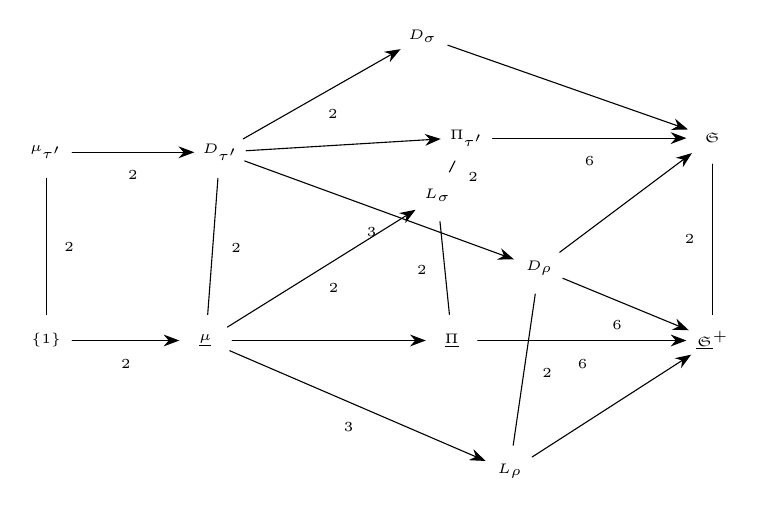
\begin{tikzpicture}[x=1mm,y=1mm,line cap=round,line join=round,font=\scriptsize]
\node[inner sep=1pt] at (7.6,-22.3) {\tiny $\mu_{\tau'}$};
\node[inner sep=1pt] at (29.7,-22.3) {\tiny $D_{\tau'}$};
\node[inner sep=1pt] at (61,-20.5) {\tiny $\Pi_{\tau'}$};
\node[inner sep=1pt] at (92.2,-20.5) {\tiny $\mathfrak S$};
\node[inner sep=1pt] at (7.6,-46.2) {\tiny $\{1\}$};
\node[inner sep=1pt] at (27.8,-46.2) {\tiny $\underline\mu$};
\node[inner sep=1pt] at (59.1,-46.2) {\tiny $\underline\Pi$};
\node[inner sep=1pt] at (92.2,-46.2) {\tiny $\underline{\mathfrak S}^+$};
\node[inner sep=1pt] at (55.4,-7.6) {\tiny $D_\sigma$};
\node[inner sep=1pt] at (57.3,-27.8) {\tiny $L_\sigma$};
\node[inner sep=1pt] at (70.2,-37) {\tiny $D_\rho$};
\node[inner sep=1pt] at (66.5,-62.8) {\tiny $L_\rho$};
\draw[-{Stealth[length=2mm]}] (10.9,-22.3) -- (26.4,-22.3);
\node[inner sep=1pt] at (18.6,-25.2) {\tiny $2$};
\draw[-{Stealth[length=2mm]}] (10.9,-46.2) -- (24.5,-46.2);
\node[inner sep=1pt] at (17.7,-49.2) {\tiny $2$};
\draw (7.6,-42.9) -- (7.6,-25.6);
\node[inner sep=1pt] at (10.5,-34.3) {\tiny $2$};
\draw (28.1,-42.9) -- (29.4,-25.6);
\node[inner sep=1pt] at (31.7,-34.5) {\tiny $2$};
\draw[-{Stealth[length=2mm]}] (32.6,-20.6) -- (52.6,-9.2);
\node[inner sep=1pt] at (44,-17.5) {\tiny $2$};
\draw[-{Stealth[length=2mm]}] (33,-22.1) -- (57.7,-20.6);
\draw[-{Stealth[length=2mm]}] (32.8,-23.4) -- (67,-35.9);
\node[inner sep=1pt] at (48.9,-32.4) {\tiny $3$};
\draw[-{Stealth[length=2mm]}] (30.6,-44.5) -- (54.5,-29.6);
\node[inner sep=1pt] at (44.1,-39.5) {\tiny $2$};
\draw[-{Stealth[length=2mm]}] (31.2,-46.2) -- (55.8,-46.2);
\draw[-{Stealth[length=2mm]}] (30.9,-47.5) -- (63.4,-61.5);
\node[inner sep=1pt] at (46,-57.2) {\tiny $3$};
\draw (58.8,-24.8) -- (59.5,-23.4);
\node[inner sep=1pt] at (61.8,-25.4) {\tiny $2$};
\draw (57.6,-31.1) -- (58.8,-42.9);
\node[inner sep=1pt] at (55.3,-37.3) {\tiny $2$};
\draw (66.9,-59.5) -- (69.7,-40.3);
\node[inner sep=1pt] at (71.2,-50.3) {\tiny $2$};
\draw[-{Stealth[length=2mm]}] (64.3,-20.5) -- (88.9,-20.5);
\node[inner sep=1pt] at (76.6,-23.4) {\tiny $6$};
\draw[-{Stealth[length=2mm]}] (58.6,-8.7) -- (89.1,-19.4);
\draw[-{Stealth[length=2mm]}] (72.8,-35) -- (89.6,-22.4);
\draw[-{Stealth[length=2mm]}] (73.2,-38.3) -- (89.2,-44.9);
\node[inner sep=1pt] at (80.1,-44.3) {\tiny $6$};
\draw[-{Stealth[length=2mm]}] (69.3,-61) -- (89.5,-48);
\draw[-{Stealth[length=2mm]}] (62.4,-46.2) -- (88.9,-46.2);
\node[inner sep=1pt] at (75.7,-49.2) {\tiny $6$};
\draw (92.2,-23.8) -- (92.2,-42.9);
\node[inner sep=1pt] at (89.3,-33.3) {\tiny $2$};
\end{tikzpicture}
\end{document}
